\subsection{Dalvik Executionable File Format} \label{subsection:android-dex}
As explained in subsection~\ref{subsection:foundation-android-package}, Android applications are distributed using dex bytecode which is compiled from Java bytecode.
Dalvik bytecode is suited to run on the ARM architecture.
It supports direct mapping from dex registers to the 32 bit registers of the ARM processor.
The instructions are 16 bit mutliples, which makes the dex bytecode less compact than Java bytecode with its 8 bit instructions.
The 16 bit instructions result in 218 valid opcodes which have a dest-source ordering for its arguments. \cite{androidDalvik}
In case there are 64 bit values, adjacent registers are used to store it.
\newline
Similar to Java bytecode, instructions are not stored inside the method but as a reference pointing to the variable.
While in Java each class has its constants, like numbers, strings and identifier names, grouped together in heterogenous pool (see figure figure~\ref{fig:java}, left side), Dalvik bytecode uses one pool for each type.
When compiling Java bytecode to Dalvik bytecode,
the heterogenous pools of each Java class are merged together in one global pool for each type (see figure figure~\ref{fig:java}, right side).
In this process, duplicates in a pool are removed, which reduces memory need for constant but increases the number of references.
This is most effective for strings.
A decrease of the memory footprint of up to 44\% compared to the \gls{jar} is possible.
\newline
\begin{figure}[h]
    \centering
    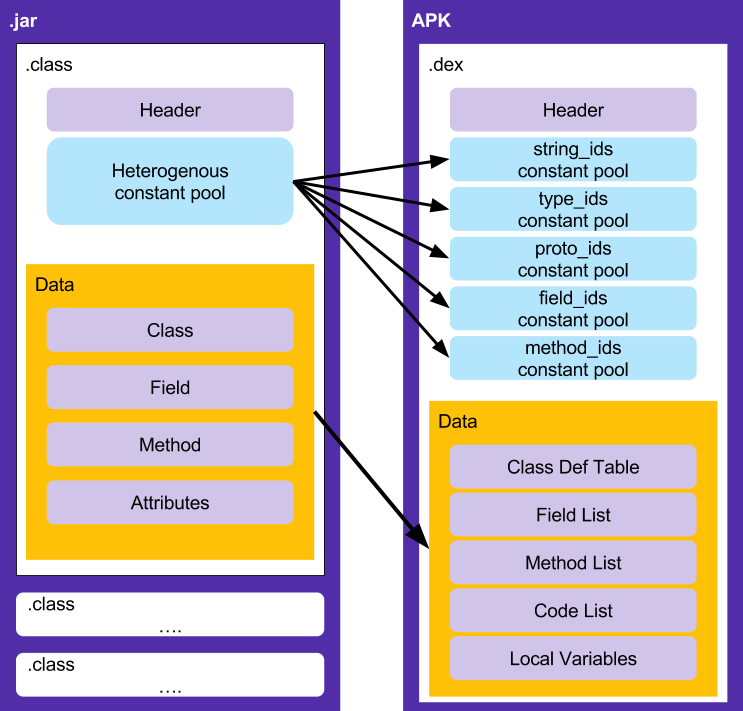
\includegraphics[width=0.5\textwidth]{data/java.png}
    \caption{\gls{jar} to \gls{apk} transformation \cite{googleDalvik}}
    \label{fig:java}
\end{figure}
The compiled \gls{dex} file has the the structure seen in figure~\ref{fig:dex} on the left.
Most important parts of the header are the checksum and the signature.
The checksum contains the Adler32 checksum of the \gls{dex} file, including everything except the magic and this field.
It is used to detect whether the file is corrupt.
The signature contains the SHA-1 signature of the content of the file, except the magic, checksum and this field.
The field is used to unqiuely identify the file.
When the file is modified, both values have to be updated.
\cite{developersDalvik} \cite{ehringerDalvik}
\newline
\begin{figure}[h]
    \centering
    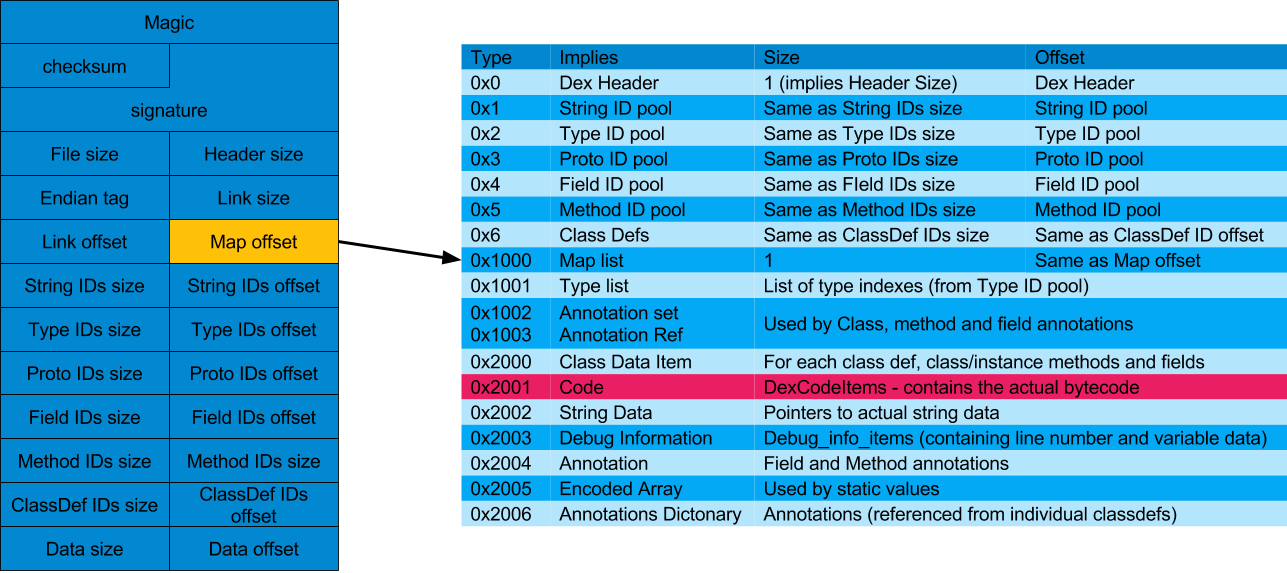
\includegraphics[width=0.8\textwidth]{data/dex.png}
    \caption{\gls{dex} file format \cite{andevconDalvikART}}
    \label{fig:dex}
\end{figure}
Dex bytecode supports optimization, upon installation improvements for the underlying architecture can be applied to the bytecode.
The resulting \gls{dex} file is called \gls{odex}.
The optimization is executed by a program called \textit{dexopt} which is part of the Android platform.
The semantics of the two files is the same, but the \gls{odex} file has the better performance.
\newline
Like Java bytecode, \gls{dex} bytecode has a serious flaw.
Since bytecode is pretty simple and contains a lot of meta information, decompilation can be succesfully done and the result is easily understandable.
At the same time, protection is rarely applied by the developers.
This makes these applications an easy target for reverse engineering.
